\chapter{Bifurcations of fixed points}
\section{Local nonlinear dynamics near fixed points}
We are interested in the local nonlinear dynamics around fixed points. Consider
\begin{align}
	\dot{x}=f(x);\quad f\in \mathcal{C}^{r},r \geq 1; \quad f(p) = 0, \numberthis \label{eq:4star}
\end{align}
i.e. $p$ is a fixed point of the dynamical system. The linearized system at $p$ is
\begin{align}
	\dot{y} = Df(p)y,\ y\in \mathbb{R}^{n},\ Df(p)\in \mathbb{R}^{n \times n}. \numberthis \label{eq:4sstar}
\end{align}
The linearization has the eigenvalues $\lambda_1, \ldots, \lambda_n \in \mathbb{C}$ with multiplicities counted. Corresponding to these eigenvalues are the eigenvectors $e_1,\ldots,e_n \in \mathbb{C}^{n}$, including generalized eigenvectors for when the algebraic multiplicity is greater than the geometric multiplicity. The eigenvector $e_j$ is real when $\lambda_j \in \mathbb{R}$.

\begin{definition}
The following subspaces are invariant for the linearized dynamical system:
\begin{enumerate}
	\item The \emph{stable subspace}
		\begin{align}
			\boxed{
				E^{S} =  \textrm{span} _{j}\left \{  \textrm{Re} (e_j),  \textrm{Im} (e_j):\  \textrm{Re} (e_j) < 0\right\},
			}
		\end{align}
	\item The \emph{unstable subspace}
		\begin{align}
			\boxed{
				E^{U} =  \textrm{span} _{j}\left \{  \textrm{Re} (e_j),  \textrm{Im} (e_j):\  \textrm{Re} (e_j) > 0\right\},
			}
		\end{align}
	\item The \emph{center subspace}
		\begin{align}
			\boxed{
				E^{C} =  \textrm{span} _{j}\left \{  \textrm{Re} (e_j),  \textrm{Im} (e_j):\  \textrm{Re} (e_j) = 0\right\}.
			}
		\end{align}
\end{enumerate}

\end{definition}
\begin{remark}[]
	Note here that the following facts hold
	\begin{enumerate}
		\item $E^{C}= \emptyset$ if and only if $p$ is hyperbolic,
		\item $E^{U,S}$ and $E^{C}$ are invariant subspaces of \eqref{eq:4sstar} by construction,
		\item Solutions of \eqref{eq:4sstar} in $E^{S}$ (resp. $E^{U}$) decay to $y=0$ as $t \to \infty$ (resp. $t \to - \infty$). 
	\end{enumerate}
	
\end{remark}

We now discuss what happens to these subspaces in the nonlinear system \eqref{eq:4star}.
\begin{theorem}[Center Manifold Theorem] \label{thm:center_mfd}
	The following hold:
	\begin{enumerate}
		\item There exists a unique \emph{stable manifold} $W^{S}(p)$ for \eqref{eq:4star}, such that
	\begin{itemize}
		\item $W^{S}(p)$ is a $\mathcal{C}^{r}$ manifold (surface), tangent to $E^{S}$ at $p$ with $ \textrm{dim } W^{S}(p) =  \textrm{dim } E^{S}$,
		\item $W^{S}(p)$ is invariant for \eqref{eq:4star} and for $x\in W^{S}(p)$ we have 
			\begin{align}
				\| F^{t}(x)-p \| \leq K_{S} \exp\left[ t \left( \max_{ \textrm{Re} (\lambda_j) < 0}( \textrm{Re} (\lambda_j)) + \varepsilon_S \right) \right]
			\end{align}
	 for $t\geq 0$, $0 < \varepsilon_S \ll 1$, and  $\| x- p\|$ small enough.
	\end{itemize}
			
		\item There exists a unique \emph{unstable manifold} $W^{U}(p)$ for \eqref{eq:4star}, such that
	\begin{itemize}
		\item $W^{U}(p)$ is a $\mathcal{C}^{r}$ manifold (surface), tangent to $E^{U}$ at $p$ with $ \textrm{dim } W^{U}(p) =  \textrm{dim } E^{U}$,
		\item $W^{U}(p)$ is invariant for \eqref{eq:4star} and for $x\in W^{U}(p)$ we have 
			\begin{align}
				\| F^{t}(x) -p\| \leq K_{U} \exp\left[ t \left( \max_{ \textrm{Re} (\lambda_j) > 0}( \textrm{Re} (\lambda_j)) + \varepsilon_U \right) \right]
			\end{align}
	 for $t\leq 0$, $0 < \varepsilon_U \ll 1$, and  $\| x- p\|$ small enough.
	\end{itemize}
			
\item There exists a (not necessarily unique) \emph{center manifold} $W^{C}(p)$ for \eqref{eq:4star}, such that
	\begin{itemize}
		\item $W^{C}(p)$ is a $\mathcal{C}^{r-1}$ manifold (surface), tangent to $E^{C}$ at $p$ with $ \textrm{dim } W^{C}(p) =  \textrm{dim } E^{C}$,
	\end{itemize}
			
	\end{enumerate}
	
\end{theorem}
The geometry of these manifolds and their corresponding subspaces are sketched in Fig. \ref{fig:mfds_def}.
\begin{figure}[h!]
	\centering
	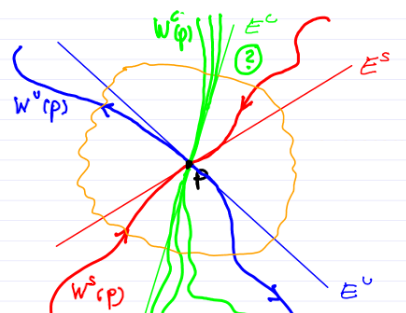
\includegraphics[width=0.6\textwidth]{figures/ch3/1manifolds_def.png}
	\caption{A sketch of the stable (red), unstable (blue), and center manifolds (green), along with their respective linear subspaces, that are invariant under the linearized dynamics. Note the existence of multiple center manifolds and the unique unstable/stable manifolds.}
	\label{fig:mfds_def}
\end{figure}

Notice that Theorem \ref{thm:center_mfd} does not state anything  about the asymptotic dynamics on the center manifold, in contrast to that of the unstable and stable manifolds. This means that the overall dynamics depends crucially on the center manifold. In the case when $W^u=\emptyset$, even the stability type of the fixed point is determined by $W^C(p)$. This is why it will be the subject of further investigations.

\section{The center manifold}
\begin{ex}[Uniqueness of the center manifold]
	Since Theorem 4.2 gave no guarantees on the uniqueness of the center manifold, now we explore this non-uniqueness in an example.
	\begin{align}
\begin{dcases}
	\dot{x} = x^2 \\
	\dot{y} = -y.
\end{dcases}
	\end{align}
	First, linearize at the origin to find the linearized dynamics
	\begin{align}
		A = Df(0) = 
		\begin{pmatrix}
			0 & 0 \\ 0 & -1
		\end{pmatrix}
		.
	\end{align}
	The linearized dynamics is illustrated in Fig. \ref{fig:cmfd_lin_ex}. We find the invariant subspaces
	\begin{align}
		E^{C} =  \textrm{span}\left\{ 
			\begin{pmatrix}
				1 \\ 0 
			\end{pmatrix}
		\right\};\quad
		E^{S} =  \textrm{span}  \left\{
			\begin{pmatrix}
				0 \\ 1
			\end{pmatrix}
		\right\}; \quad
		E^{U} = \emptyset.
	\end{align}
	The nonlinear manifolds are illustrated with the invariant subspaces from the linearization in Fig. \ref{fig:cmfd_lin_ex}.
	\begin{figure}[h!]
		\centering
		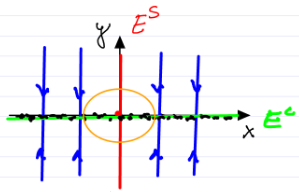
\includegraphics[width=0.45\textwidth]{figures/ch3/2cmfd_lin_ex.png}
		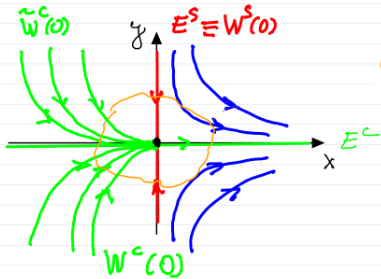
\includegraphics[width=0.4\textwidth]{figures/ch3/3cmfd_nonlin_ex.png}
		\caption{Left: The linearized dynamics around the origin. Right: The nonlinear phase portrait. }
		\label{fig:cmfd_lin_ex}
	\end{figure}
	Observe that there exist infinitely many center manifolds which are all invariant and all tangent to $E^{C}$ at the origin. We also see that although the fixed point at the origin is stable in the linearized system, it is unstable in the nonlinear system.
\end{ex}

We now present a method to calculate $W^C(p)$ in general cases.
\begin{enumerate}
	\item Consider 
		\begin{align}
			\dot{z} = F(z); \quad F(0) = 0;\quad z \in \mathbb{R}^{c+d};\quad F \in \mathcal{C}^{r},
		\end{align}
	where $c$ represents the number of center directions at the origin ($ \textrm{dim }E^{C}$) and $d$ denotes the remaining directions ($ \textrm{dim } E^{U} +  \textrm{dim } E^{S}$).
	\item Now block-diagonalize the linearization. This consists of four steps
		\begin{enumerate}
			\item First linearize the dynamics to find $\dot{z} = Mz + \mathcal{O}(\|z\|^2)$ with $M = DF(0) \in \mathbb{R}^{(c+d) \times (c+d)}$.
			\item Define the transformation matrix
				\begin{align}
					T=
					\begin{bmatrix}
						a_1 & \ldots & a_c & b_1 & \ldots & b_d	
					\end{bmatrix}
				=
				\begin{bmatrix}
					\textrm{basis in } E^{C} &  \textrm{basis in } E^{U} \oplus E^{S}
				\end{bmatrix}
				.
				\end{align}
			\item Pass to the basis from the transformation matrix by introducing a new set of coordinates as $z = T \xi$
				\begin{align}
					\dot{\xi} = T^{-1}\dot{z} = T^{-1}MT \xi + T^{-1}\mathcal{O}(\| T\xi\|^2) = 
					\begin{pmatrix}
						A & 0 \\
						0 & B
					\end{pmatrix}
					\xi + \mathcal{O}(\| \xi \| ^2).
				\end{align}
			The matrices $A$ and $B$ are elements of $\mathbb{R}^{c \times c}$ and $\mathbb{R}^{d \times d}$ respectively.	
		\item Let $\xi = 
			\begin{pmatrix}
				x \\ y
			\end{pmatrix}
			\in \mathbb{R}^{c}\times \mathbb{R}^{d}$, the $x$-coordinates are aligned with $E^{C}$ and the $y$-coordinates are perpendicular to them. We then find
			\begin{align}
				\dot{x} = Ax + f(x,y);\quad \dot{y} = By + g(x,y), \numberthis \label{eq4:trafod_eqn}
			\end{align}
			for $f,g \in \mathcal{C}^{r}$ and $f,g = \mathcal{O}(\|x\|^2, \|y\|^2, \|x\|\|y\|)$. The geometry in these coordinates is depicted in Fig. \ref{fig:cmfd_trafo_geom}. The center manifold is given by
			\begin{align}
				W^{C}(0) = \left\{ (x,y) \in U:\ y = h(x)\right\}
			\end{align}
			for $h:\mathbb{R}^{c} \to \mathbb{R}^{d}$ and $ h \in \mathcal{C}^{r-1}$ as in the theorem.
			\begin{figure}[h!]
				\centering
				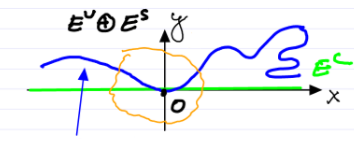
\includegraphics[width=0.4\textwidth]{figures/ch3/4cmfd_trafo_geom.png}
				\caption{The geometry of the nonlinear system in the transformed coordinates aligned with the invariant subspaces of the linearization. The blue arrow points to the center manifold $W^{C}(0)$.}
				\label{fig:cmfd_trafo_geom}
			\end{figure}
		\end{enumerate}
	\item Now we use the invariance of $W^{C}(0)$, i.e. for all $t$, it holds that $y(t) = h(x(t))$. With this we find
		\begin{align}
			\dot{y} = Dh(x(t)) \dot{x}(t).
		\end{align}
		We can now substitute $\dot{x}$ and $\dot{y}$ from \eqref{eq4:trafod_eqn} to get the following nonlinear partial differential equation (PDE) for $h(x)$
\begin{align}
	\boxed{
		Bh(x) + g(x, h(x)) = Dh(x) \left[ Ax + f(x, h(x))\right] \numberthis \label{eq4:1star}.
	}
\end{align}
In addition to \eqref{eq4:1star} being nonlinear, the boundary conditions are also  unknown. Therefore there is little hope for solving it analytically.
\item Instead take the Taylor expansion of \eqref{eq4:1star} to approximate the solution
	\begin{align}
		h(x) = \underbrace{h(0)}_{=0} + \underbrace{Dh(0)}_{=0}x + \frac{1}{2} \underbrace{D^2h(0)}_{3- \textrm{tensor} } \otimes x \otimes x + \mathcal{O}(\|x \| ^3),
	\end{align}
	where the first two terms are 0 due to the tangency to $E^{C}$ at $0$. We therefore have that $h = O(x^2)$ and we are justified in seeking $W^C(0)$ in this form. We can then restrict the system to the center manifold by substituting $y = h(x)$ to get the reduced dynamics as 
	\begin{align}
		\boxed{
			\dot{x}=Ax+f(x,h(x)).
		}
	\end{align}
\end{enumerate}

\begin{ex}[Finding the center manifold]
	Consider the dynamical system
	\begin{align}
		\begin{dcases}
			\dot{x}=xy \\
			\dot{y}=-y+\alpha x.
		\end{dcases}	
	\end{align}
	First we linearize at $(0,0)$ to get 
	\begin{align}
		M =
		\begin{pmatrix}
			[0] & [0] \\
			[0] & [-1]
		\end{pmatrix}
	\end{align}
	which is already in block-matrix form. The dimensions of the stable, unstable, and center subspaces of the linearization are 1, 0, and 1 respectively. Hence the stability type depends on the dynamics on the center manifold $W^{C}(0)$. We now look for a parameterization of $W^{C}(0)$ in the form
	\begin{align}
		h(x) = ax^2 + bx^3 + cx^4 + \mathcal{O}(x^5).
	\end{align}
	Since the right-hand side of the dynamical system was $\mathcal{C}^\infty$, this expansion could formally be continued to any order. However, the expansion will not converge as that would imply the uniqueness of the center manifold. In this example, we work with a finite, order 4 truncation. Now use the invariance (the PDE \eqref{eq4:1star} we derived above) to find
	\begin{align}
		\dot{y} = h'(x)\dot{x} = \left[2ax+3bx^2 + 4cx^3 + \mathcal{O}(x^4) \right] x \left[ax^2+bx^3+cx^4 + \mathcal{O}(x^5) \right]. \numberthis \label{eq4:one}	
	\end{align}
	On the other hand, from the dynamical system we know
	\begin{align}
		\dot{y}=-h(x) + \alpha x^2 =(\alpha - a) x^2 -bx^3 - cx^4 + \mathcal{O}(x^5). \numberthis \label{eq4:two}
	\end{align}
	Equations \eqref{eq4:one} and \eqref{eq4:two} must hold for all $x$ small enough, therefore the coefficients of equal powers of $x$ in these two equations must match.
	\begin{align}
		\mathcal{O}(x^2)&:\ \alpha = a\\
		\mathcal{O}(x^3)&:\ b=0 \\
		\mathcal{O}(x^4)&:\ 2a^2 = -c.
	\end{align}
	Therefore we find 
	\begin{align}
		\boxed{
	h(x) =\alpha x^2 - 2\alpha^2x^4 + \mathcal{O}(x^5).}
	\end{align}
	Then the dynamics on $W^{C}(0)$ becomes
	\begin{align}
		\boxed{
			\dot{x}= xh(x) = \alpha x^3(1-2\alpha x^2) + \mathcal{O}(x^6). \numberthis \label{eq4:2star}
		}
	\end{align}
	The dynamics is depicted in Fig. \ref{fig:cmfd_alpha_diff}. For $\alpha > 0$ the origin is unstable, meanwhile for $ \alpha <0$ the origin is asymptotically stable.
	\begin{figure}[h!]
		\centering
		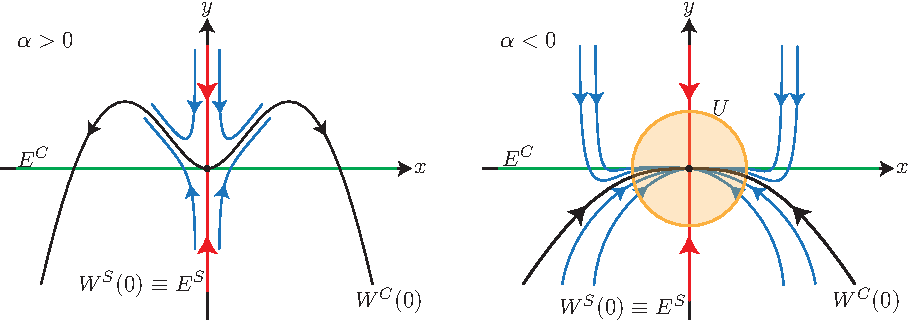
\includegraphics[width=0.8\textwidth]{figures/ch3/5cmfd_alpha_diff}
		\caption{Left: The nonlinear dynamics on the center manifold for $\alpha > 0$. Right: The nonlinear dynamics on the center manifold for $\alpha < 0$.}
		\label{fig:cmfd_alpha_diff}
	\end{figure}
	
	The full local stable manifold for $\alpha <0$ is $\overline{W}^{S}(0)=U$ and it is of dimension 2. The difference between $\overline{W}^{S}(0)$ and $W^{S}(0)$ is that in general the decay rate in $\overline{W}^{S}(0)-W^{S}(0)$ is generally weaker than the rate guaranteed in the Center Manifold Theorem. 

\begin{remark}[]
	The $\mathcal{O}(x^5)$ truncation has two hyperbolic fixed points at $x = \pm \frac{1}{\sqrt{2 \alpha} }$, however the full system has no such fixed points. The reason for this is that away from the origin, the $\mathcal{O}(x^6)$ terms are no longer guaranteed to be small relative to the $\mathcal{O}(x^5)$ terms, and the truncation this far away from 0 is not justified.
\end{remark}
\end{ex}

After this example we would like to explore if the concept of the center manifold is robust, as the existence of eigenvalues with $ \textrm{Re} (\lambda_i) = 0$ is not. We will explore this in an example.

\begin{ex}[Perturbing the previous example]
	Consider the following perturbed dynamical system
	\begin{align}
		\begin{dcases}
			\dot{x} = xy + \varepsilon x \\
			\dot{y} = -y + \alpha x^2
		\end{dcases}
;\quad |\varepsilon | \ll 1.
	\end{align}
The linearization of this system yields
\begin{align}
	\begin{dcases}
		\dot{x} = \varepsilon x \\
		\dot{y} = -y.
	\end{dcases}
\end{align}
Now the center manifold disappears as the center subspace $E^{C}$ disappears for $\varepsilon>0$!
\end{ex}

\section{Center manifolds depending on parameters}
We begin with the setup
\begin{align}
	\begin{dcases}
		\dot{x} = Ax + f(x,y,\varepsilon) \\
		\dot{y} = By + g(x,y,\varepsilon)
	\end{dcases}
;\quad x \in \mathbb{R}^{c},\ y \in \mathbb{R}^{d},\ 0\leq \varepsilon \ll 1;\\
f,g \in \mathcal{C}^{r},\ f,g=\mathcal{O}(\|x\|^2, \|y\|^2, \|x\|\|x\|, {\varepsilon \|x\|, \varepsilon \|y\|} ).
\end{align}
The order $\varepsilon \|x\|$ and $\varepsilon \|y\|$ terms are due to the perturbation of the linear part. Now assume $ \textrm{Re} (\lambda _j(A))= $ for $j=1,\ldots,c$ (the center directions) and $ \textrm{Re} (\lambda _j(B)) \neq  $ for $j=1,\ldots,d $ (the hyperbolic directions). Next, rewrite $\tilde{x}=
\begin{pmatrix}
	x \\ \varepsilon
\end{pmatrix}
$ and $\tilde{y}=y$ to obtain the system
\begin{align}
	\begin{dcases}
		\dot{\tilde{x}} = \tilde{A}\tilde{x} + \tilde{f}(\tilde{x}, \tilde{y}) \\
		\dot{\tilde{y}} = \tilde{B}\tilde{y} + \tilde{g}(\tilde{x}, \tilde{y}) 
	\end{dcases}
	;\quad \tilde{A}=
	\begin{pmatrix}
		A & 0 \\ 0 & 0	
	\end{pmatrix}
	\in \mathbb{R}^{(c+1)\times (c+1)}; \quad \tilde{f} =
	\begin{pmatrix}
		f \\ 0
	\end{pmatrix}. \numberthis \label{eq4:unostar}
\end{align}
Here, $\tilde{g}=g$ and $\tilde{B}=B$. Further, note that $ \textrm{span} \left\{
	\begin{pmatrix}
		x \\0
	\end{pmatrix}
\right\}$ is an invariant subspace for $\tilde{A}$. The eigenvalues of $\tilde{A}$ are the same as those of $A$ and an additional $0$, thus there are $c+1$ center directions and $d$ hyperbolic directions. Applying the center manifold theorem to the fixed point $0 \in \mathbb{R}^{c+1+d}$ of \eqref{eq4:unostar} we obtain that there exists a $\tilde{W}^{C}(0)$ $\mathcal{C}^{r-1}$ manifold tangent to $E^{C}$ at $
\begin{pmatrix}
	\tilde{x} \\ \tilde{y}
\end{pmatrix}
= 
\begin{pmatrix}
	0 \\ 0
\end{pmatrix}
$ which is invariant and is of dimension $c+1$. The geometry of this manifold is illustrated in Fig. \ref{fig:pert_cent_mfd}. Note in the figure that there is no dynamics in the $\varepsilon$ direction, as $\dot{\varepsilon}=0$ and that $(x,y)=(0,0)\in \mathbb{R}^{c+d}$ remains a fixed point for $\varepsilon\neq 0$.
\begin{figure}[h!]
	\centering
	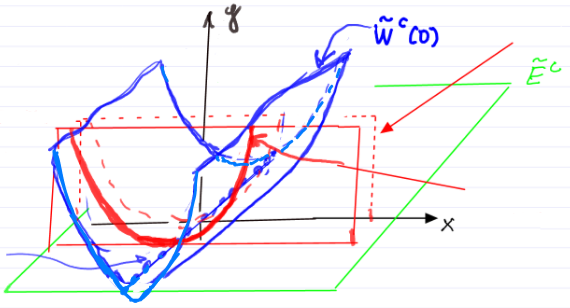
\includegraphics[width=0.7\textwidth]{figures/ch3/6pert_cent_mfd.png}
	\caption{Geometry of the center manifold with the perturbation. The straight red arrow designates the cut at $\varepsilon=0$ which is equal to $W^{C}(0)$, the squiggly red arrow points at the continuation of the center manifold from $\varepsilon=0$ to $\varepsilon \neq 0$.}
	\label{fig:pert_cent_mfd}
\end{figure}

Computing $\tilde{W}^{C}(0)$ is done in a similar fashion as before. We use the center manifold theorem to get	
\begin{align}
	\tilde{y} = y= \tilde{h}(\tilde{x}) = \tilde{h}(x,\varepsilon) = \mathcal{O}(\|x\|^2, \varepsilon \|x\|, \varepsilon^2) = \mathcal{O}(\|x\|^2, \varepsilon \|x\|).
\end{align}
The order $\varepsilon^2$ term was dropped as $x=0$ must remain a fixed point. The function $h$ describes the graph of $W^{C}_{\varepsilon}(0)$. Then the reduced dynamics on $W^{C}_{\varepsilon}(0)$ is
\begin{align}
	\boxed{
		\dot{x} = Ax + f(x, \tilde{h}(x, \varepsilon), \varepsilon).
}
\end{align}
This can then be applied to the perturbed example from above.

\begin{ex}[Revisting the perturbation]
	Recall the dynamical system
	\begin{align}
		\begin{dcases}
			\dot{x} = xy + \varepsilon x\\
			\dot{y} = -y + \alpha x^2.
		\end{dcases}
	\end{align}
	We have the persisting fixed point at $(x,y)=(0,0)\in \mathbb{R}^{c+d}$	and the system is already in standard form with 
	 \begin{align}
		 A=0;\quad B=-1;\quad f(x,y,\varepsilon) = xy + \varepsilon x;\quad g(x,y,\varepsilon) = -\alpha x^2.
	\end{align}
	We apply the center manifold theorem and get the existence of $W^{C}_{\varepsilon}(0)$ for $|\varepsilon|\ll 1$. This manifold satisfies
	 \begin{align}
		 y = \tilde{h}(x,\varepsilon) = ax^2 + bx\varepsilon + c\varepsilon^2
		 +dx^3 + ex^2 \varepsilon +j x\varepsilon^2 + k\varepsilon ^3
		 +lx^4. \ldots \numberthis \label{eq4:juanstar}
	\end{align}
	The term $c\varepsilon^2$ must be equal to 0 for all $\varepsilon$ such that the fixed point persists, therefore $c=0$. Next the invariance $y(t) = \tilde{h}(x(t)), \varepsilon)$ is used, taking the time derivative on both sides yields
	\begin{align}
	\dot{y} = \left[2ax + b\varepsilon + \mathcal{O}(2) \right]
	\underbrace{\left[\mathcal{O}(3) + \varepsilon x \right]} _{=\dot{x}  \textrm{ from ODE and \eqref{eq4:juanstar} }}
		= 2a \varepsilon x^2 + b\varepsilon^2 x  + \mathcal{O}(4).
	\end{align}
	The $\mathcal{O}(n)$ designates terms of total degree $n$, for example $x^n$ or $x^{n-k}\varepsilon^{k}$. From the ODE we find
	\begin{align}
		\dot{y} = -y + \alpha x^2 
		= -ax^2 -bx\varepsilon - c\varepsilon^2 - dx^3 - e x^2 \varepsilon - j x \varepsilon^2 -k \varepsilon^3 - \mathcal{O}(4) + \alpha x^2.
	\end{align}
	Comparing equal powers in these two equations we find
	\begin{align}
		\mathcal{O}(x^2)&:\ 0 = \alpha -a; \quad
		&\mathcal{O}(\varepsilon^2)&:\ 0=-c;\quad
         	&\mathcal{O}(x\varepsilon)&:\ 0=-b; \\
		\mathcal{O}(\varepsilon^3)&:\ 0=-t; \quad
		&\mathcal{O}(x^3)&:\ 0=-d;\quad
		&\mathcal{O}(x^2\varepsilon)&:\ 2a=-e;\\
		\mathcal{O}(x\varepsilon^2)&:\ b=-j.
	\end{align}
	Thus the shape of $W^{C}_{\varepsilon}(0)$ is given by 
	\begin{align}
		y = \tilde{h}(x,\varepsilon) = \alpha(1-2\varepsilon)x^2+ \mathcal{O}(4).
	\end{align}
	The dynamics on $W^{C}_{\varepsilon}(0)$ is
	\begin{align}
		\dot{x} = \varepsilon x + \alpha(1-2\varepsilon)x^3 + \mathcal{O}(5).
	\end{align}
	We can see there is no substantial change in the shape of $W^{C}_{\varepsilon}(0)$ relative to the $\varepsilon=0$ case. The stability type is determined by the sign of $\varepsilon$ and a two time-scale dynamic persists.	
\end{ex}
From this example we may still wonder what effect the higher order terms have on the center manifold.

\section{Normal forms}
For a general treatment see \cite{GuckenheimerHolmes}, here we will consider one example to illustrate the idea originally coming from Poincaré.

\begin{ex}[Reduced dynamics on 1-dimensional manifold]
	Consider the following 1-dimensional dynamical system
	\begin{align}
		\dot{x}=x(\mu -x^2)+x^4;\quad 0 \leq| \mu| \ll 1.
	\end{align}
	The fixed points are at $x=0$ and the roots of $g_\mu (x) = \mu -x^2 + x^3$. This function $g_\mu $ is illustrated in Fig. \ref{fig:gmu_roots}.
	\begin{figure}[h!]
		\centering
		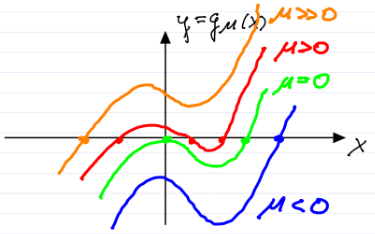
\includegraphics[width=0.4\textwidth]{figures/ch3/7gmu_roots.png}
		\caption{The functions $g_\mu $ for different values of $\mu $.}
		\label{fig:gmu_roots}
	\end{figure}
	By plotting $x$ as a function of $\mu $ such that $g_{\mu }(x)=0$ we get the \emph{bifurcation diagram} as shown in Fig. \ref{fig:gmu_bifurc}.
	\begin{figure}[h!]
		\centering
		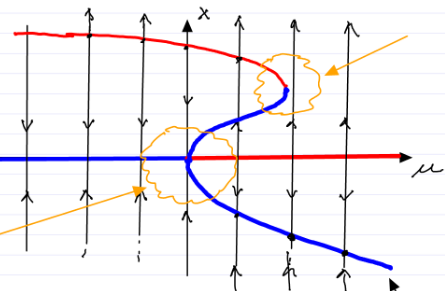
\includegraphics[width=0.6\textwidth]{figures/ch3/8gmu_bifurc.png}
		\caption{Bifurcation diagram for the 1-dimensional dynamical system. Red and blue demarcate if the fixed point at the given $(x, \mu)$ pair is stable (blue) or unstable (right). The arrow on the right points towards a \emph{fold bifurcation} and the arrow on the left towards a \emph{pitchfork bifurcation}. The curve is given by implicitly solving $g_{\mu}(x)=0$.}
		\label{fig:gmu_bifurc}
	\end{figure}

	The fold bifurcation (see caption of Fig. \ref{fig:gmu_bifurc}) is created by quartic (order 4) terms, which become more important away from the origin. The pitchfork bifurcation is already captured by the cubic truncation. We would like to know when the truncation captures the full dynamics correctly near the origin. Poincaré showed that, in fact, the truncated system is topologically equivalent to the full system near the origin by using a change of coordinates to remove $\mathcal{O}(4)$ terms.

	\begin{enumerate}
		\item 		
	Let $x =y + h_4(y)= y+ay^4 + \mathcal{O}(y^5) $, which is near the identity near the origin, hence it is also invertible near the origin (by the Implicit Function Theorem). Further, this preserves the ODE up to the $\mathcal{O}(3)$ terms.  
\item
	Plug in $x(t)$ and $y(t)$ and take the derivative with respect to time to get
	\begin{align}
		\dot{x} = \dot{y}(1+4ay^3 + \mathcal{O}(y^4)).
	\end{align}
\item 
Now use the ODE and find
\begin{align}
	\dot{x}=\mu x - x^3 +x^4 = \mu (y+ay^4)-(y+ay^4)^3 + (y-ay^4)^5 + \ldots.
\end{align}
\item
	Combine the previous two steps and calculate
\begin{align}
	\dot{y}= \left[1 + 4ay^3 + \mathcal{O}(y^4)\right]^{-1} \left[\mu y + a \mu y^4 - y^3+y^4 + \mathcal{O}(5)\right].	
\end{align}
At this point recall the alternating series (it could be verified with Taylor expansion)
\begin{align}
	\frac{1}{1+z} = 1-z + \mathcal{O}(z^2);\quad 0 \leq |z| \ll 1.
\end{align}
We also note that a generalized result holds for an operator $A \in R^{m \times m }$, which could be used in higher dimensional calculations. This is referred to as the Neumann series. Applying this to the left term in the formula for $\dot{y}$ yields
\begin{align}
	\left[1 + 4ay^3 + \mathcal{O}(y^4)\right]^{-1}=1 - 4ay^3 + \mathcal{O}(y^4). 
\end{align}
Therefore we find
\begin{align}
	\dot{y} &= \mu y - y^3 + y^4\underbrace{(-4a \mu  +a \mu +1)}_{ \textrm{choose }a  \textrm{ such that this }  =0} + \mathcal{O}(y^5).
\end{align}
We may now choose the parameter $a$ to make the coefficient of the quartic term 0. The $a$ that fulfills this is $a=\frac{1}{3 \mu }$, using this we find
\begin{align}
	\boxed{
		\dot{y} = \mu y-y^3+\mathcal{O}(y^5).
	}
\end{align}
This transformation has removed the quartic terms from the equation.
\item
	Now we remove the $\mathcal{O}(y^5)$ terms similarly. First set 
	\begin{align}
		y = \xi + h_5(\xi) = \xi + b \xi^5 + \mathcal{O}(\xi^6)
	\end{align}
	and then continue as before, but with $y$ now playing the role of $x$ and $\xi$ playing the role of $y$.
\item The successive sequence of near identity coordinate changes turns out to converge usually. In general, it depends on the type of problem, sometimes resonant terms are not removeable and must stay as they are crucial to the dynamics. These resonant terms depend only on the linear part of the RHS, for more information see Chapter 3 of \cite{GuckenheimerHolmes}.
	\end{enumerate}
Thus 
\begin{align}
	\boxed{
\dot{x} = \mu x - x^3	
}
\end{align}
is the \emph{normal form} for the ODE for the study of bifurcations at the origin for $0 \leq \mu \ll 1$. It is topologically equivalent to the full system near $x=0$ and captures the pitchfork bifurcation.
\end{ex}

\section{Bifurcations}
A \emph{bifurcation} is a qualitative change in the dynamical system
\begin{align}
	\boxed{
		\dot{x} =f(x, \mu );\quad x \in \mathbb{R}^{n};\quad \mu \in \mathbb{R}^{p}.
	} \numberthis \label{eq4:astar}
	\end{align}
	Linear stability analysis led to reducing to the center manifold (depending on parameters). From there we moved to normal forms which enable the analysis of qualitative dynamics under varying parameters. 
	\begin{definition}[Local bifurcation]
		A \emph{local bifurcation} is a qualitative change in the behavior of a system near a non-hyperbolic equilibrium. More precisely, a \emph{bifurcation} occurs in \eqref{eq4:astar} at $\mu = \mu _0$ near the fixed point $x=0$ if there exists \underline{no} neighborhood of $x=0$ in which $\dot{x}=f(x, \mu _0)$ is topologically equivalent to \underline{all} systems $\dot{x} = f(x, \mu )$ for $\|\mu -\mu _0\|$ small enough.
	\end{definition}
	This idea of a bifurcation can be illustrated by a bifurcation surface which separates the space of dynamical systems into components. Within each component the dynamical systems are topologically equivalent, however elements from separate components are not. This is sketched in Fig. \ref{fig:bif_surf_def}.
	\begin{figure}[h!]
		\centering
		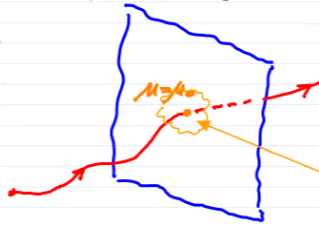
\includegraphics[width=0.5\textwidth]{figures/ch3/9bif_surf_def.png}
		\caption{Illustration of a bifurcation surface (blue). The near side of the surface is one component, and the far side the other. The red path is a family of dynamical systems $\{\dot{x} = f(x,\mu )\}_{\mu \in \mathbb{R}^{p}}$, going through the bifurcation point $\mu_0$. Around this point, a neighborhood as outlined in the definition is sketched in orange.}
		\label{fig:bif_surf_def}
	\end{figure}

We wish to understand what happens in the case that a given family of dynamical systems is nongeneric (atypical). For instance in the case that the family forms a tangency to the bifurcation surface, in which case a bifurcation does not take place, hence the family of dynamical systems is not general enough to capture all possible dynamics.

\begin{ex}[Nongeneric family of dynamical systems]
	In comparison to the family taken previously consider
	\begin{align}
		 \dot{x} = -a^2 x -x^3;\quad \mu =-a^2\leq 0.
	\end{align}
	For every $\mu $ which we consider, there is only one fixed point $x=0$ and it is stable for all values of $\mu $. However, we have unwittingly missed the full picture, as for $\mu >0$ there are three fixed points, one of which are unstable. This situation is shown in Fig. \ref{fig:nongen_ds}.
	\begin{figure}[h!]
		\centering
		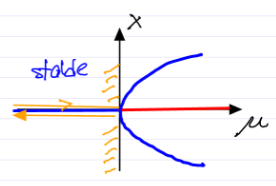
\includegraphics[width=0.4\textwidth]{figures/ch3/10nongen_ds.png}
		\caption{A nongeneric family of dynamical systems. We only see what happens to the left of the $x$-axis, and miss everything to the right, hence our family is tangent to the bifurcation surface.}
		\label{fig:nongen_ds}
	\end{figure}
\end{ex}

This idea of nongeneric families motivates our next definition, which is also depicted in Fig. \ref{fig:univ_unfold_def}.
\begin{definition}[Universal unfolding]
	A paramaterized family of dynamical systems crossing all nearby topological equivalence classes as the parameters vary is called a \emph{universal unfolding}.
\end{definition}
\begin{figure}[h!]
	\centering
	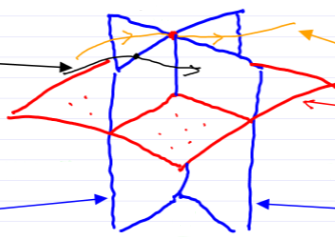
\includegraphics[width=0.45\textwidth]{figures/ch3/11univ_unfold_def.png}
	\caption{An example of universal unfolding (red) for the red bifurcation point which crosses the four topologically equivalent classes (components) created by the two bifurcation surfaces (blue). Furthermore, a nonuniversal unfolding is shown by the yellow 1-dimensional path at the top. Another universal unfolding in for the black bifurcation point, is shown by the 1-dimensional black family.}
	\label{fig:univ_unfold_def}
\end{figure}

\begin{definition}[Codimension of a bifurcation] The \emph{codimension of a bifurcation} is the minimum number of parameters required for a universal unfolding. Thus a more degenerate bifurcation requires a larger codimension.
\end{definition}

\section{Codimension 1 bifurcations}
We begin by considering different types of center manifolds. We start by classifying these by the number of zero eigenvalues which appear in the linearization.
\begin{enumerate}
	\item \textbf{Single zero eigenvalue} Our system is as follows
		\begin{align}
			\dot{y} = f(y, \mu),\ y \in \mathbb{R}^{n},\ \mu\in \mathbb{R}^{p};\quad f(0,0)=0;\quad  \textrm{dim }E^{C}=1\implies  \textrm{dim } W^{C}_{\mu }(0)=1.  
		\end{align}
		Thus we have a single zero eigenvalue, an example eigenvalue constellation which fulfills this is given in Fig. \ref{fig:1zero_eigv}.
		\begin{figure}[h!]
			\centering
			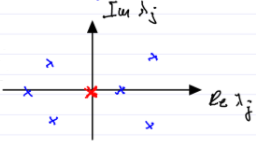
\includegraphics[width=0.4\textwidth]{figures/ch3/12onezero_eigv.png}
			\caption{An example eigenvalue constellation with a single zero eigenvalue.}
			\label{fig:1zero_eigv}
		\end{figure}
		The universal unfolding (generally parameterized by the normal form on $W^{C}_{\mu }(0)$) is given by
		\begin{align}
			\boxed{
				\dot{x} = \tilde{\mu }\pm x^2;\quad x \in \mathbb{R};\quad \tilde{\mu } \in\mathbb{R}.
			}
		\end{align}
		This is a codimension 1 bifurcation, i.e. only 1 parameter is needed for the universal unfolding. Hence we find a bifurcation diagram as shown in Fig. \ref{fig:codim1_bif}. This is called a \emph{fold} or \emph{saddle node} bifurcation, in this example it is \emph{supercritical} as we show the $-x^2$ case. \emph{Subcriticality} occurs when the diagram is mirrored with respect to the $x$-axis, i.e. when the fixed points disappear for $\mu > 0$. The sign which is actually used is problem dependent.
		\begin{figure}[h!]
			\centering
			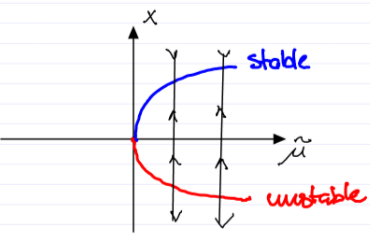
\includegraphics[width=0.35\textwidth]{figures/ch3/13codim1_bif.png}
			\caption{A codimension 1 fold bifurcation, which is supercritical.}
			\label{fig:codim1_bif}
		\end{figure}
		\begin{remark}[]
			\emph{Hysteresis} is the dependence of the output on past input and is often related to interplay between two such fold bifurcations as shown in Fig. \ref{fig:hysteresis}.
		\begin{figure}[h!]
			\centering
			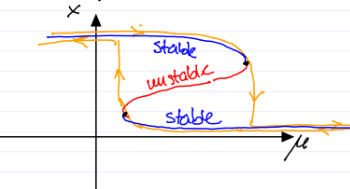
\includegraphics[width=0.4\textwidth]{figures/ch3/14hysteresis.png}
			\caption{An example of hysteresis caused by two interacting fold bifurcations. In this case, the hysteresis is a result of purely deterministic dynamics, no additional memory (or delay) terms were needed.}
			\label{fig:hysteresis}
		\end{figure}
		
		\end{remark}
		
	\item \textbf{Single zero eigenvalue \& origin remains a fixed point} 	
		Now we have more conditions and our setup is as follows
		\begin{align}
			\dot{y} = f(y, \mu),\ y \in \mathbb{R}^{n},\ \mu\in \mathbb{R}^{p};\quad f(0,\mu )=0,\ \forall \mu ;\quad  \textrm{dim }E^{C}=1\implies  \textrm{dim } W^{C}_{\mu }(0)=1.  
		\end{align}
		Thus we have the additional degeneracy $D_{\mu }f(0,0)=0$. We get the universal unfolding 
		\begin{align}
			\dot{x} = \tilde{\mu }x \pm x^2 = x (\tilde{\mu } \pm x);\quad x \in \mathbb{R};\quad \tilde{\mu} \in \mathbb{R}.	
		\end{align}
		This so called \emph{transcritical bifurcation} is depicted in Fig. \ref{fig:transcrit_bif}. In such bifurcations the observed stable state does not vary until the bifurcation, after which it begins to vary linearly.
		\begin{figure}[h!]
			\centering
			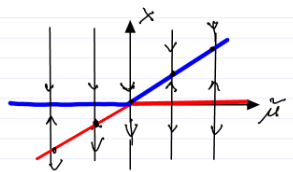
\includegraphics[width=0.35\textwidth]{figures/ch3/15transcrit_bif.png}
			\caption{A transcritical bifurcation.}
			\label{fig:transcrit_bif}
		\end{figure}
	\item \textbf{Single zero eigenvalue, origin remains a fixed point, \& RHS is an odd function} 
		We have the same setup as previously, with the additional condition that
		\begin{align}
			f(y,0) = - f(-y,0)\implies D^2_{y}f(y,0) = -D^2_{y}f(-y,0) \implies D^2_{y}f(0,0) = 0.
		\end{align}
	This leads to the universal unfolding 
	\begin{align}
		\dot{x} = \tilde{\mu } x \pm x^3;\quad x \in \mathbb{R};\quad \mu \in \mathbb{R}.
	\end{align}
	This type of bifurcation is called a \emph{pitchfork bifurcation}. It is \emph{supercritical} for the $+x^3$ case (cf. Fig. \ref{fig:pitchfork_bif}), and subcritical for the $-x^3$ case. The actual sign is problem dependent.
\begin{figure}[h!]
	\centering
	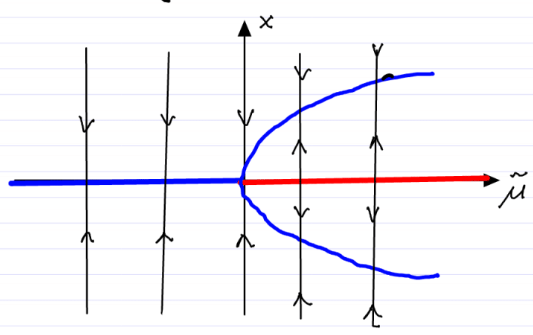
\includegraphics[width=0.35\textwidth]{figures/ch3/16pitchfork_bif_A.png}
	\caption{A supercritical (i.e with a $+$ sign) pitchfork bifurcation.}
	\label{fig:pitchfork_bif}
\end{figure}
\item \textbf{Purely imaginary pair of eigenvalues} 
	Now we have the following setup, with the eigenvalue constellation shown in Fig. \ref{fig:imag_pair_eigv}. 
	\begin{align}
		f(0,0)=0;\quad  \textrm{dim } E^{C}=2; \quad \lambda_n(0)= \overline{\lambda }_{n-1}(0) = \pm i\omega \neq 0.
	\end{align}
\begin{figure}[h!]
	\centering
	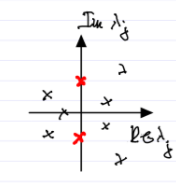
\includegraphics[width=0.25\textwidth]{figures/ch3/17imag_pair_eigv.png}
	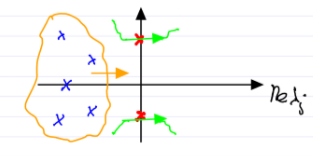
\includegraphics[width=0.55\textwidth]{figures/ch3/18loss_of_stab_pair_imag.png}
	\caption{Left: Eigenvalue constellation for purely imaginary pair of eigenvalues. Right: Loss of stability in oscillating system as the pair of eigenvalues cross the imaginary axis.}
	\label{fig:imag_pair_eigv}
\end{figure}
Such constellations are common in oscillatory systems at the loss of stability. This loss of stability is sketched in the right pane of Fig. \ref{fig:imag_pair_eigv}. The reduced system dynamics on the 2-dimensional $W^{C}(0)$ for $\mu =0$ is
\begin{align}
	\begin{pmatrix}
		\dot{u} \\ \dot{v}
	\end{pmatrix}
	= 
	\begin{pmatrix}
		0 & -\omega \\
		\omega & 0
	\end{pmatrix}
	\begin{pmatrix}
		u \\ v
	\end{pmatrix}
	 +
	 \begin{pmatrix}
		 \tilde{f}(u,v) \\
		 \tilde{g}(u,v)
	 \end{pmatrix}
	 . \numberthis \label{eq4:loss_stab_cent_mfd}
\end{align}
The coordinates $(u,v)$ correspond to the basis given by $\left[  \textrm{Re} (e_n),  \textrm{Im} (e_n)\right]$. The normal form on $W^{C}_{\mu }(0)$ is
\begin{align}
	\dot{r}&= r\left(d(\mu )+a(\mu )r^2\right) + \mathcal{O}(r^5); &&d(\mu )=  \textrm{Re} (\lambda _n(\mu )) \\
	\dot{\theta } &= \omega(\mu ) + e( \mu )r^2 + \mathcal{O}(r^4);&&\omega(\mu )=  \textrm{Im} (\lambda _n(\mu )).
\end{align}
The functions $a$ and $e$ depend on the given $\tilde{f}$ and $\tilde{g}$ (thereby also on $f$). We then define
\begin{align}
	d_0 &= \frac{d}{d\mu } \textrm{Re} \left.\left[ \lambda _n(\mu ) \right] \right|_{\mu =0}; 
		\quad \omega_0= \textrm{Im} (\lambda_n(0 ))\\
		a_0 &= a(0) = \frac{1}{16}\left. \left[\tilde{f}_{uuu} + \tilde{f}_{uvv} + \tilde{g}_{uuv} + \tilde{g}_{vvv}\right] \right|_{(u,v)=0} \\
		    &\quad +\frac{1}{16\omega } \left. \left[\tilde{f}_{uv}(\tilde{f}_{uu}+ \tilde{f}_{vv}) - \tilde{g}_{uv}(\tilde{g}_{uu}+\tilde{g}_{vv}) - \tilde{f}_{uu} \tilde{g}_{uu} + \tilde{f}_{vv}\tilde{g}_{vv}\right]\right|_{(u,v)=0}.
\end{align}
Note that we must start from the standard form \eqref{eq4:loss_stab_cent_mfd}. 
\end{enumerate}
Building on this last case, we explore the extended center manifold in the next theorem.

\begin{theorem}[Hopf-Bogdanov]
	Assume the following
	\begin{enumerate}
		\item The eigenvalues $\lambda_n$ and $\overline{\lambda}_{n} $ do cross the imaginary axis for $\mu \neq 0$, i.e. $d_0 \neq 0$.
		\item The leading order nonlinearity in $\dot{r}$ is nonzero, i.e. $a_0 \neq 0$.
			Then there exists a \underline{unique} extended center manifold $W^{C}_{\mu }(0)$ for $0 \leq \mu  \ll 1$, on which the dynamical system is locally topologically equivalent to the universal unfolding 
			\begin{align}
			\boxed{
			\dot{r} = r \left( d_0 \mu + a_0 r^2\right); \quad 
			\dot{\theta}= \omega_0 + e_0r^2 + b_0 \mu ,}
			\end{align}
		for $b_0, e_0 \in \mathbb{R}$.	
	\end{enumerate}
\end{theorem}

From here we explore two cases for the signs of $d_0$ and $a_0$.
\begin{enumerate}
	\item First, when each are strictly positive $d_0, a_0 >0$. This yields a subcritical pitchfork bifurcation in $r$ and a continued rotation in $\theta $. The bifurcation of $r$ and the dynamics of $u$ and $v$ for $\mu < 0 $ are illustrated in Fig. \ref{fig:case1_hb}, for $|\mu |$ and $|r|$ small enough.
		\begin{figure}[h!]
			\centering
			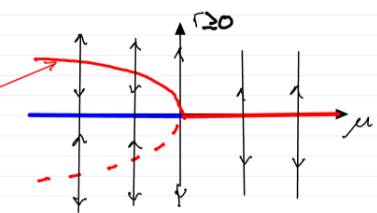
\includegraphics[width=0.45\textwidth]{figures/ch3/19case1_r_bif.png}
			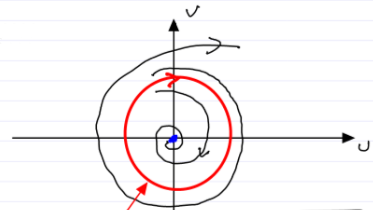
\includegraphics[width=0.45\textwidth]{figures/ch3/20case1_theta_bif.png}
			\caption{Left: The subcritical pitchfork bifurcation of $r$. The red arrow points towards the $r = \sqrt{\frac{-d_0 \mu }{a_0}}$, the symmetric negative part of this curve is dashed, as negative values of $r$ are not relevant for this problem (the radius cannot be negative). Right: The effect of $\mu <0$ on the system dynamics leading to an unstable limit cycle (red) in the $u-v$ plane.}
			\label{fig:case1_hb}
		\end{figure}
		There is an increased sensitivity to perturbation as $\mu $ increases (the domain of attraction shrinks). This is shown in Fig. \ref{fig:case1_full_bif}. Such behavior can be observed in the transition to turbulence in pipe flows. In that context, the equation is referred to as the Stuart-Landau equation.
		\begin{figure}[h!]
			\centering
			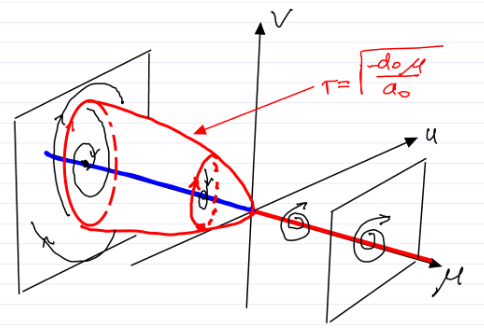
\includegraphics[width=0.6\textwidth]{figures/ch3/21case1_full_bif.png}
			\caption{The full bifurcation diagram for the dynamical system in case (i).}
			\label{fig:case1_full_bif}
		\end{figure}
	\item Next, the two coefficients have opposite signs $d_0 > 0$ and $a_0 <0$. This leads to the supercritical Hopf bifurcation and a stable limit cycle as shown in Fig. \ref{fig:case2_bif}
		\begin{figure}[h!]
			\centering
			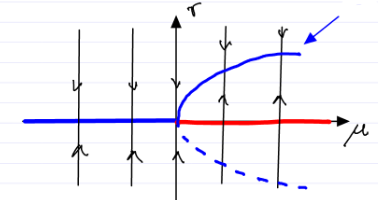
\includegraphics[width=0.5\textwidth]{figures/ch3/23case2_bif.png}
			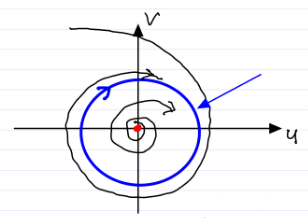
\includegraphics[width=0.4\textwidth]{figures/ch3/22case2_r_bif.png}
			\caption{Left: The bifurcation in $r$, the blue arrow designates the curve given by $r=\sqrt{\frac{-d_0 \mu }{a_0}}$, again the negative part is not relevant as the radius is always non-negative. Right: The stable limit cycle that arises for this system.}
			\label{fig:case2_bif}
		\end{figure}
	
		There is a sudden development of stable periodic oscillation as $\mu  $ is increased. Often the parameter $\mu $ is a steady speed in the system which is changed gradually. Examples of this are 
		\begin{itemize}
			\item increasing wind speed leading to bridge oscillations and collapse,
			\item increasing flight speed leading to wing flutter,
			\item increasing driving speed leading to death wobble on motorcycles.
		\end{itemize}
		
\end{enumerate}

